\documentclass[aspectratio=169]{beamer}

\usetheme{metropolis}
\usepackage{graphicx}
\usepackage{amsmath}
\usepackage{booktabs}
\usepackage{xcolor}

% Paths to existing paper assets
\graphicspath{{figures/main/}{figures/supplement/}}

\title{Causal Network Topology Predicts \\ How LLM Forecasters Revise Probabilities \\ When Presented with New Information}
\subtitle{Current Results + Proposed External Forecasting Extension}
\author{Sean Kelley}
\institute{Northeastern University \textbar{} Lab Meeting}
\date{\today}

\begin{document}

\maketitle

% ─────────────────────────────────────────────────────────────
\section{Motivation}

\begin{frame}{Where this sits}
\begin{itemize}
  \item LLMs increasingly used as forecasters on complex multi-domain questions.
  \item Prior work evaluates \emph{accuracy} against markets or ground truth.
  \item Much less is known about \emph{how} forecasts emerge — what factors the model weighs, how it updates under new evidence.
  \item Without that, forecasts remain black boxes that are hard to audit or interrogate.
\end{itemize}
\end{frame}

\begin{frame}{Central question}
\textbf{Do LLM forecasters update their probabilities in a way that is internally consistent with the causal structure they themselves elicit?}

\vspace{1em}
If yes, the elicited DAG is more than a post-hoc rationalization — it is a genuine diagnostic of the reasoning that produced the forecast.
\end{frame}

% ─────────────────────────────────────────────────────────────
\section{Method}

\begin{frame}{Pipeline}
Four stages applied to each of 116 high-complexity ForecastBench questions, across seven models.
\begin{enumerate}
  \item \textbf{Causal Forecast} — LLM produces initial probability $p_0$ and a directed causal graph $G=(V,E)$ with 6--10 factor nodes, one outcome node, and annotated mechanisms on edges.
  \item \textbf{Network Analysis} — compute betweenness centrality and outcome mediation; rank nodes into high / medium / low importance tiers.
  \item \textbf{Probe Generation} — LLM authors $\sim$21 counterfactual probes per question spanning strengthen, negate, structural challenge, and control types.
  \item \textbf{Probed Forecast} — present each probe in a fresh context; record updated probability $p_i$.
\end{enumerate}
\end{frame}

\begin{frame}{Dependent variable}
Probability shifts are mechanically bounded (a forecast of $0.9$ can move at most $+0.09$ upward), so we use the absolute log-odds shift:
\[
  |\Delta\text{logit}|_i = \left| \log\tfrac{p_i}{1-p_i} - \log\tfrac{p_0}{1-p_0} \right|
\]

\vspace{0.5em}
Primary model is a linear mixed-effects regression with question-level random intercepts and model fixed effects, fit in R using \texttt{lme4}.
\end{frame}

\begin{frame}{Two exemplar DAGs}
\centering
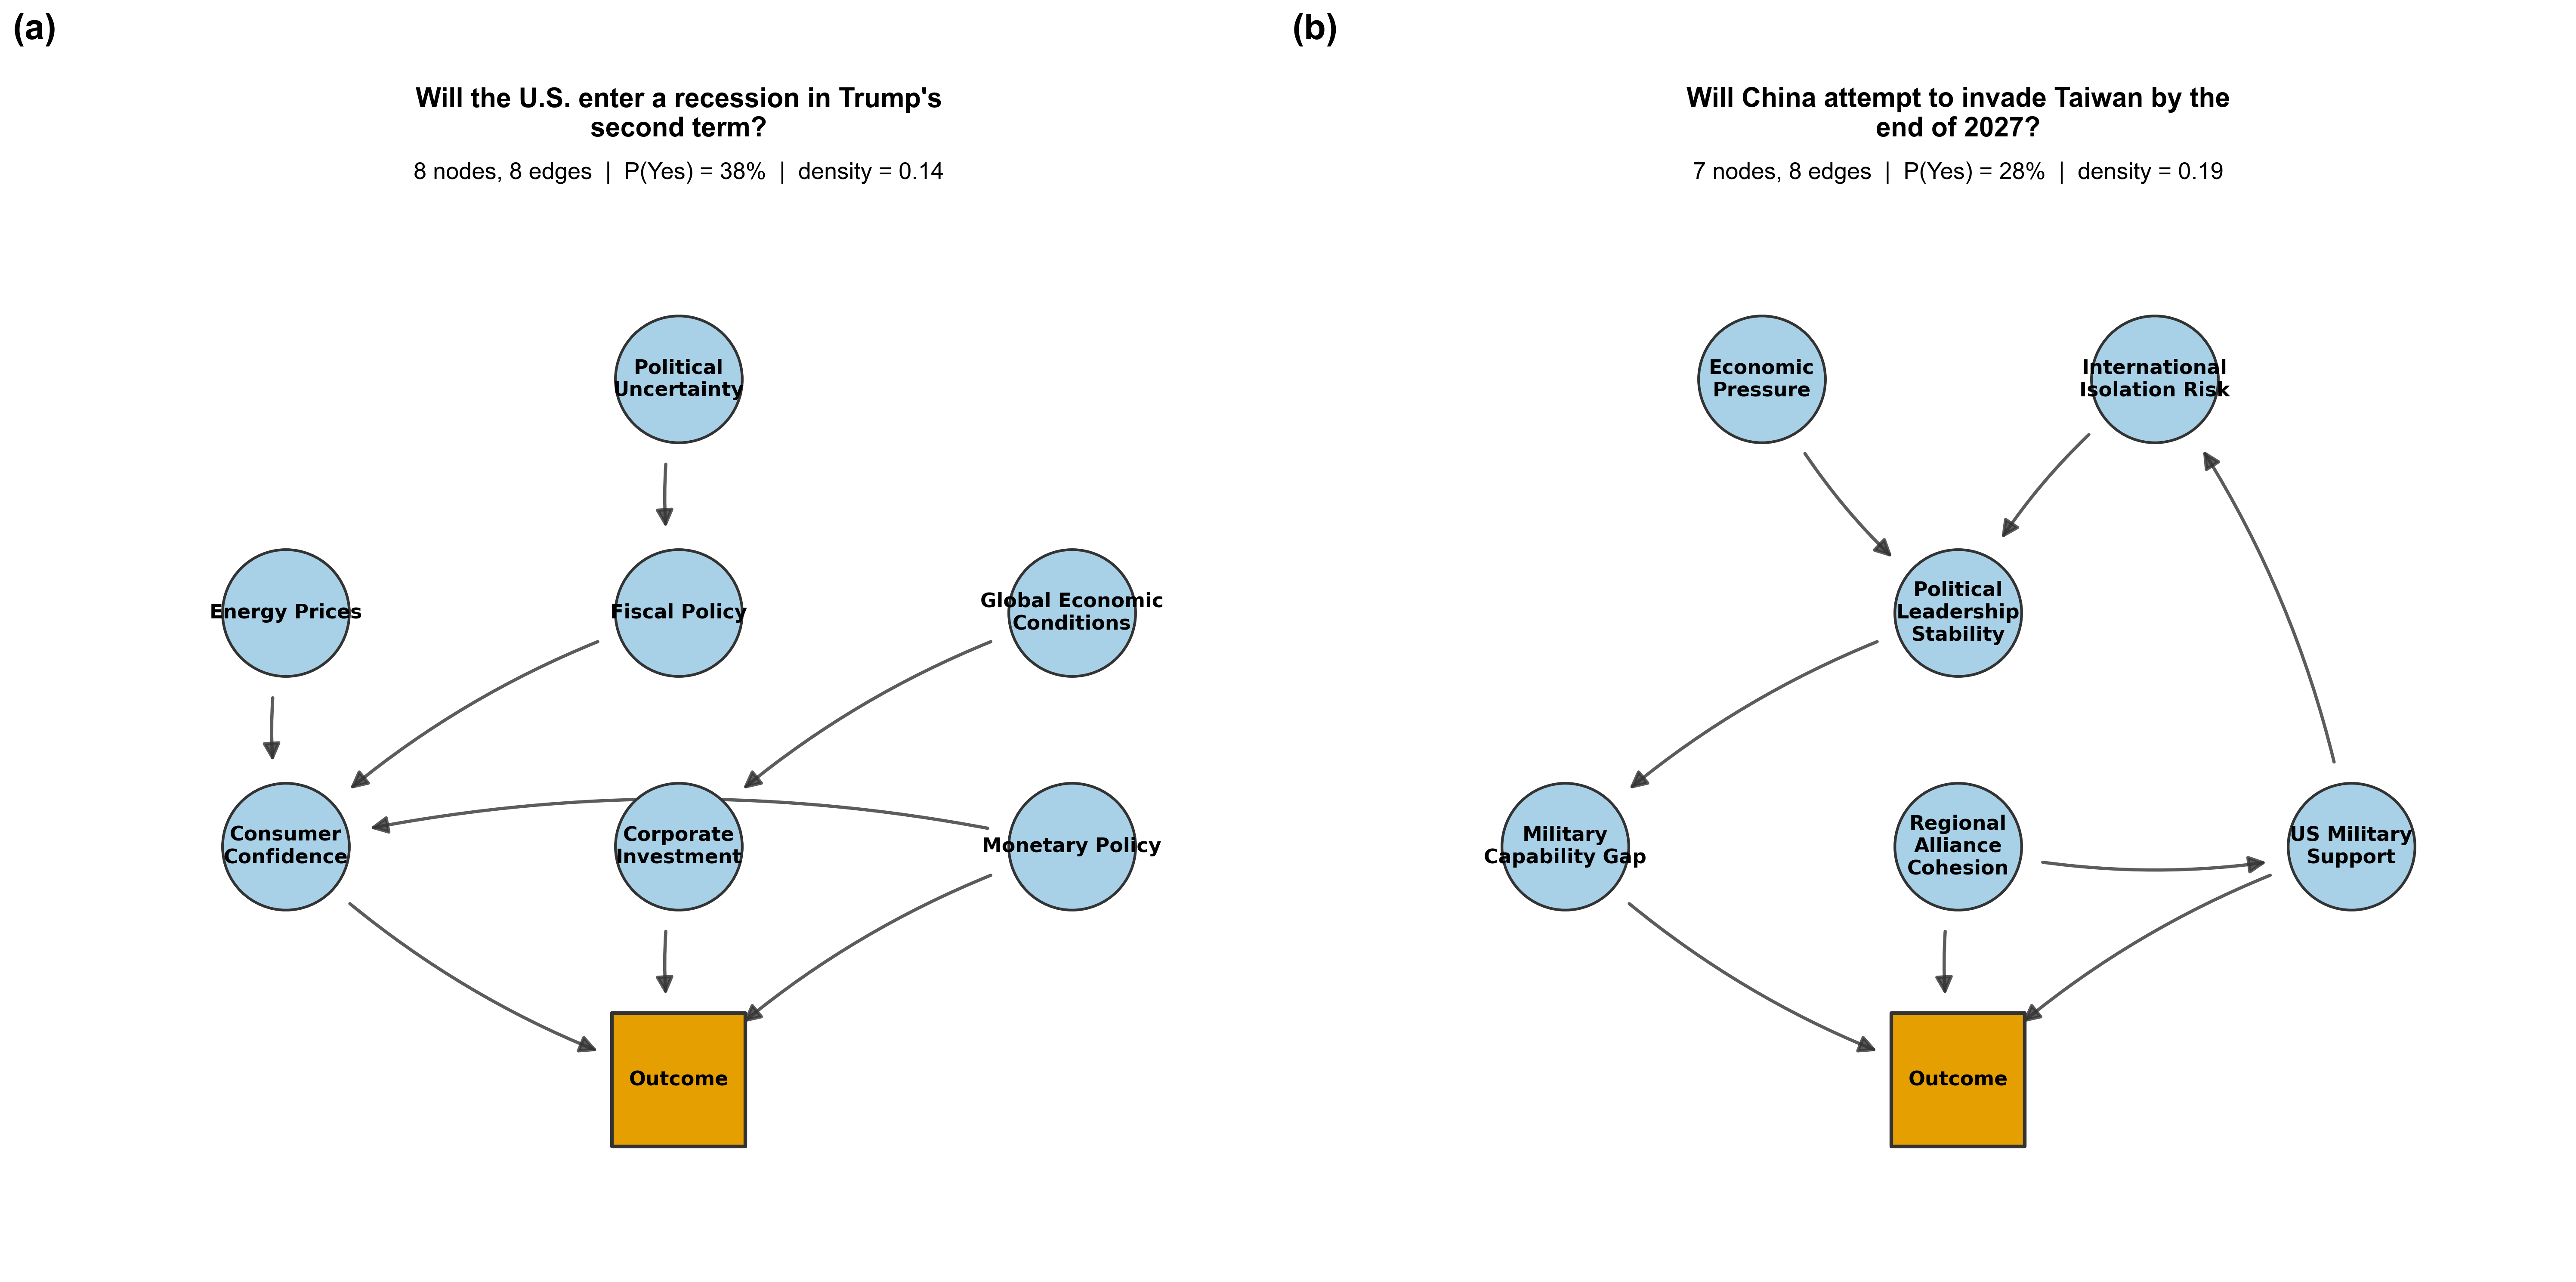
\includegraphics[width=0.88\linewidth]{exemplar_networks_combined.png}
\vspace{0.3em}

\small Left: macroeconomic question (8 nodes, 8 edges). Right: geopolitical question (7 nodes, 8 edges). Different domains, recognizable topology.
\end{frame}

% ─────────────────────────────────────────────────────────────
\section{Results}

\begin{frame}{Topology predicts probe sensitivity}
Each standard deviation of node betweenness centrality adds $0.0093$ to $|\Delta\text{logit}|$ ($p < .001$). Outcome mediation adds $0.0105$.

\vspace{0.5em}
In probability space that is $\sim$0.2 percentage points per SD at $p_0=0.5$ — small individually but cumulative across tiers. Probes on the most central factors shift probabilities 2--3 percentage points more than probes on peripheral ones.

\vspace{1em}
\centering
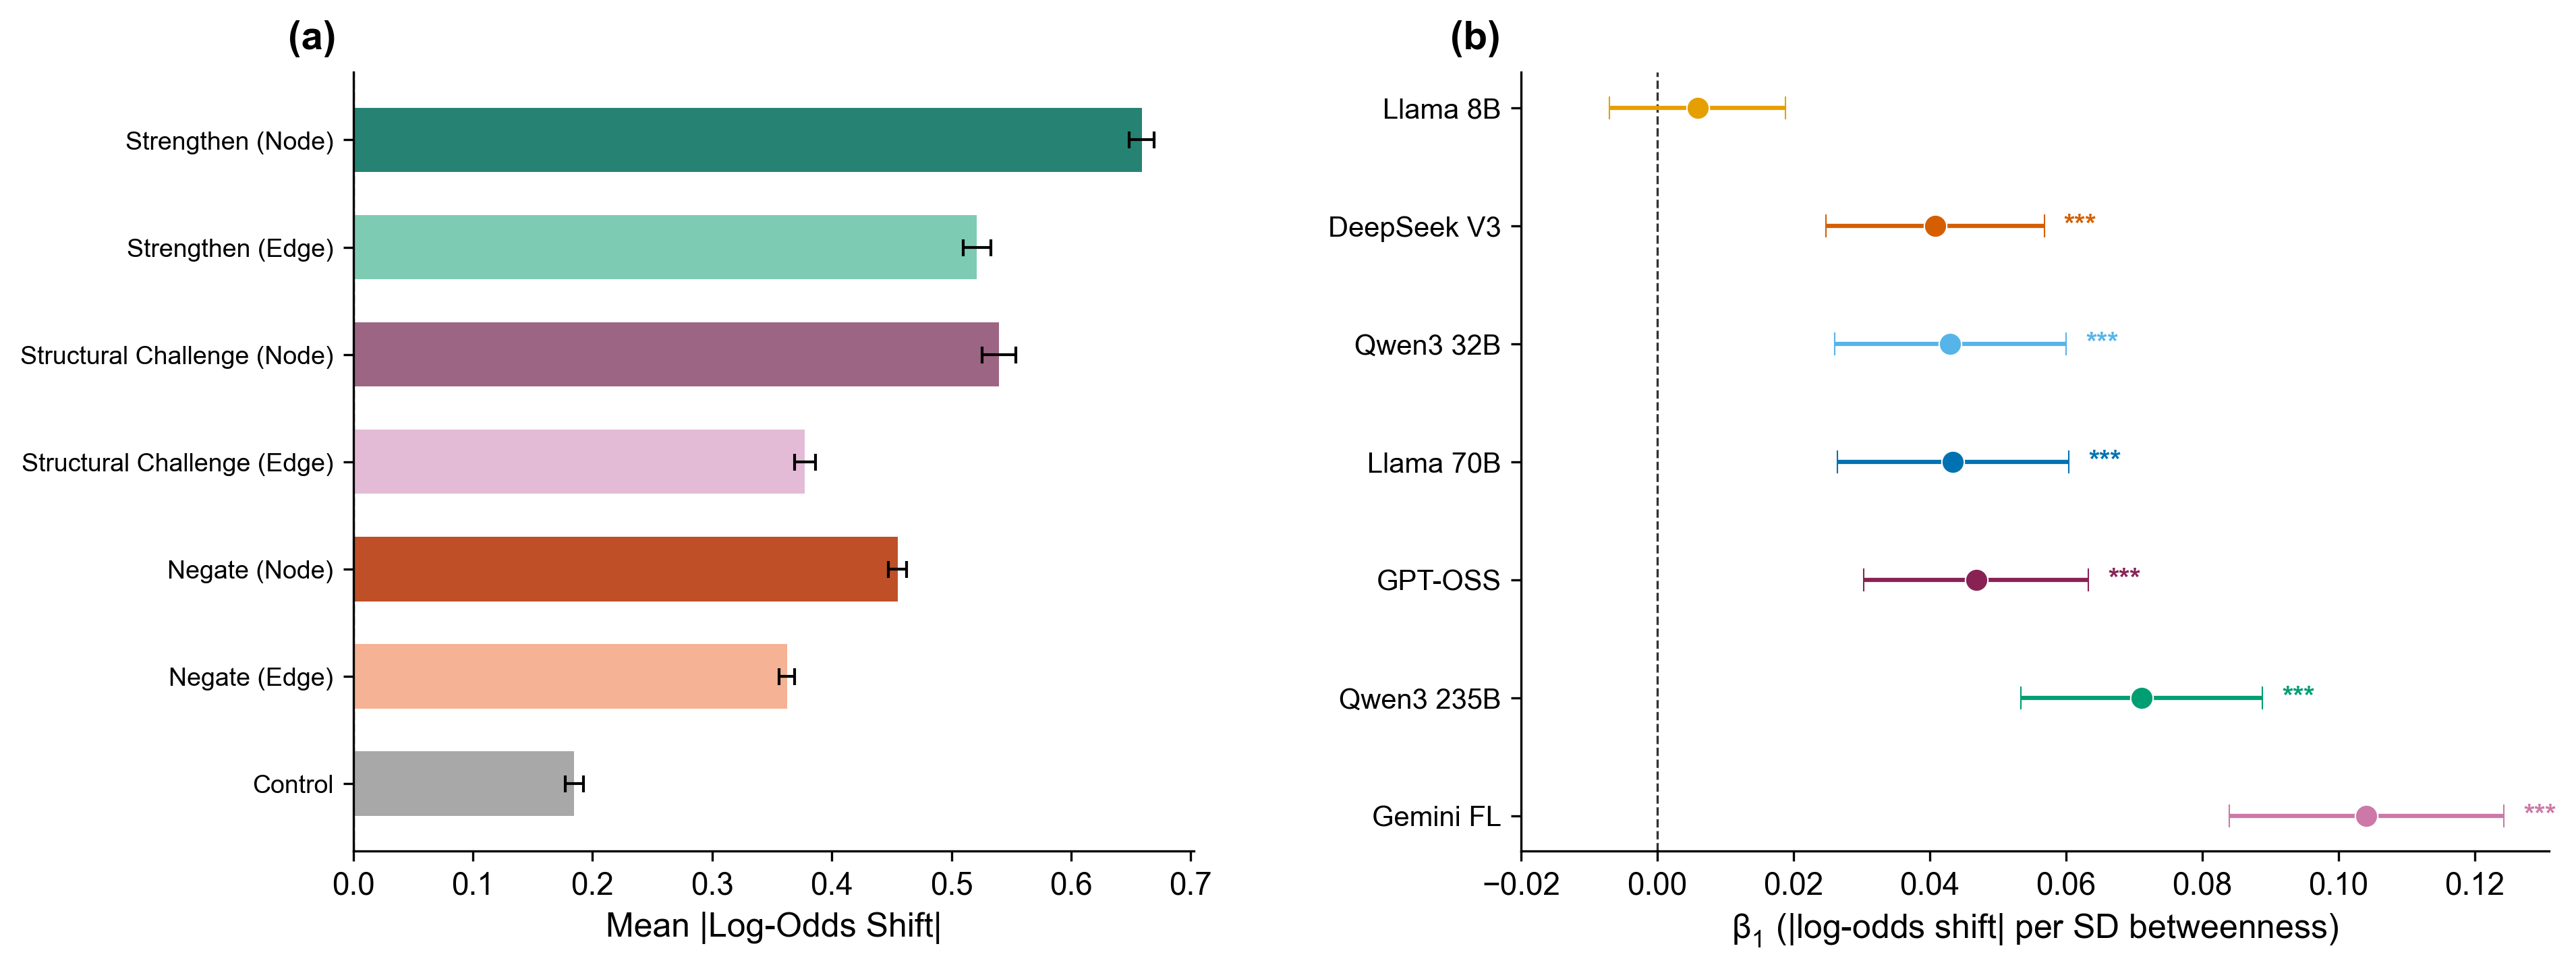
\includegraphics[width=0.95\linewidth]{probe_effects.png}
\end{frame}

\begin{frame}{The effect holds across models}
Six of seven models show a positive, significant grounding coefficient. Slopes range from $0.009$ (DeepSeek V3, Qwen3 32B) to $0.022$ (Gemini 2.5 Flash Lite). Llama 3.1 8B is the one exception.

\vspace{0.5em}
Probes targeting nodes produce larger shifts than probes targeting edges ($0.57$ vs $0.43$; $d=0.47$, $p < .001$), a pattern that holds in every model with per-model node-edge gaps ranging from $+0.07$ to $+0.25$.
\end{frame}

\begin{frame}{Reasoning covaries with the update}
\centering

\includegraphics[width=0.9\linewidth]{coherence.png}
\vspace{0.3em}

\small Judge-rated stated impact tracks $|\Delta\text{logit}|$; confident reasoning produces larger updates than hedged; Bayesian coherence shows updates shrink as $p_0$ moves from $0.5$; reasoning embeddings cluster more tightly for targeted probes than irrelevant controls.
\end{frame}

\begin{frame}{Explicit ranking and implicit topology both matter}
Models asked to rank their own factors produce rankings that align with betweenness ($\beta = -0.336$, $p < .001$).

\vspace{0.5em}
But both stated rank and betweenness independently predict $|\Delta\text{logit}|$ in a joint model ($\beta_{\text{rank}} = -0.057$, $\beta_{\text{betw}} = 0.025$; both $p < .001$, joint $R^2_m = .249$).

\vspace{0.5em}
The structural signal is partly implicit — visible in behavioral updating, not fully accessible through introspective ranking.
\end{frame}

\begin{frame}{Cross-model DAG agreement}
Same-question DAGs are more similar than a permutation null, but the absolute agreement is modest.

\vspace{0.3em}
\begin{itemize}
  \item Observed semantic nGED = 0.881, null = 0.998 ($p < .001$).
  \item Outcome nodes match across 96\% of cross-model pairs.
  \item Edge operations drive 61\% of the remaining edit mass versus 39\% for node operations.
  \item Models disagree more about causal wiring than about which factors matter.
\end{itemize}

\vspace{0.5em}
Honest framing: structural overlap exceeds chance; convergence is partial, not interchangeable.
\end{frame}

\begin{frame}{Validation checks}
Four controls in the main table plus three supplementary checks. All point the same direction.

\begin{itemize}
  \item \textbf{Persuasiveness}: importance-shift correlation survives residualizing on independent persuasiveness ratings.
  \item \textbf{Forced-ignore}: instructing the model to ignore a factor (no probe) still yields shifts scaled to that factor's centrality.
  \item \textbf{Edge rewiring}: randomizing the DAG's edges drops the grounding slope by $\sim$19\%.
  \item \textbf{Larger graphs}: doubling the node cap leaves the slope unchanged.
  \item Spurious-background contamination: 0/116. Test-retest $\rho$: 0.73--0.96. Temperature-driven nGED much smaller than inter-model divergence.
\end{itemize}
\end{frame}

\begin{frame}{What the paper establishes}
\begin{itemize}
  \item LLM forecasters update internally consistently with their own elicited causal DAGs.
  \item Node betweenness and outcome mediation both predict the magnitude of probability revision.
  \item Nodes move probabilities more than edges; direct and indirect causes contribute independently.
  \item The pattern holds across six of seven models and survives persuasiveness, rewiring, and size controls.
  \item Cross-model structural agreement is above chance but partial.
\end{itemize}

\vspace{0.7em}
\centering
Structural faithfulness: the elicited DAG is a genuine diagnostic of the reasoning behind the forecast.
\end{frame}

% ─────────────────────────────────────────────────────────────
\section{Proposed Extension: External Forecasting}

\begin{frame}{From coherence to accuracy}
The paper shows the DAG governs how a model revises its beliefs. It does not show that those revisions are \emph{better calibrated} than they would be otherwise.

\vspace{0.5em}
\textbf{Next question.} If high-betweenness factors are where the model weighs evidence most heavily, can we use that topology to guide an evidence-gathering agent and improve forecast accuracy on held-out questions?
\end{frame}

\begin{frame}{Four-condition design}
All four start from the same Stage 1 DAG and $p_0$. Equal total budget across search conditions.

\vspace{0.3em}
\begin{tabular}{@{}p{3.3cm}p{8cm}@{}}
\toprule
\textbf{Condition} & \textbf{Evidence gathering} \\
\midrule
\texttt{no\_search} & None; $p_1 = p_0$ (baseline). \\
\addlinespace
\texttt{untargeted} & Agent free-searches the question. 8 queries. \\
\addlinespace
\texttt{topology\_targeted} & Searches focused on top-3 high-betweenness factors. \\
\addlinespace
\texttt{peripheral\_targeted} & Searches focused on bottom-3 low-betweenness factors. \\
\bottomrule
\end{tabular}

\vspace{0.6em}
\small \textbf{Primary contrast}: topology vs peripheral (isolates centrality from decomposition). \\
\textbf{Secondary contrast}: topology vs untargeted (combined centrality + decomposition effect).
\end{frame}

\begin{frame}{Why the peripheral\_targeted arm?}
Without it, a topology win is ambiguous between two stories.

\vspace{0.4em}
Free-form \texttt{untargeted} queries tend to be paraphrases of the main question and return overlapping snippets. Any factor-scoped decomposition breaks that redundancy and may win for that reason alone, regardless of which factors are targeted.

\vspace{0.6em}
\texttt{peripheral\_targeted} decomposes identically to \texttt{topology\_targeted}. Same prompt, same queries per factor, same integration format. Only the factor selection differs.

\vspace{0.6em}
If topology beats peripheral, centrality is load-bearing. If they tie, decomposition was the whole story.
\end{frame}

\begin{frame}{Questions, models, scoring}
\begin{itemize}
  \item \textbf{Questions}: $\sim$500 ForecastBench instances (2x oversample) resolving 7--90 days out. Data-anchored sources: yfinance, dbnomics, FRED, ACLED, Wikipedia. Markets excluded.
  \item \textbf{Models}: five of the paper's seven (smaller models excluded by default; agentic tool-use unreliable at that scale).
  \item \textbf{Ground truth}: ForecastBench's own nightly resolution sets, idempotent re-run at each milestone.
  \item \textbf{Scoring}: Brier $(p_1 - y)^2$. Primary paired Wilcoxon of $B_{\text{peripheral}} - B_{\text{topology}}$ within (question, model). Secondary: topology vs untargeted. Supplementary LME with crossed random effects.
\end{itemize}
\end{frame}

\begin{frame}{Tiered resolution strategy}
Sources resolve on different clocks, so the experiment releases results in three milestones.

\vspace{0.4em}
\begin{tabular}{@{}p{2.2cm}p{5.5cm}p{4cm}@{}}
\toprule
\textbf{Milestone} & \textbf{Sources covered} & \textbf{Expected coverage} \\
\midrule
Week 2 \\ (preliminary) & yfinance, Wikipedia, daily FRED (rates), daily dbnomics & few dozen to 100 pairs per model \\
\addlinespace
Week 4 \\ (interim) & +ACLED weekly, FRED weekly, short-horizon dbnomics & 100--200 pairs per model \\
\addlinespace
Week 8--12 \\ (final) & +FRED monthly macro (CPI, payrolls, unemployment) & $\geq$200 pairs per model \\
\bottomrule
\end{tabular}

\vspace{0.5em}
\small Preliminary and interim are exploratory. Final milestone is the publication-grade test.
\end{frame}

\begin{frame}{Expected outcomes and what each would mean}
\begin{itemize}
  \item \textbf{Topology beats peripheral.} Centrality signal transfers from coherence to accuracy. Strongest extension of the paper's claim. Elicited DAGs become a decision tool, not just an interpretability artifact.
  \item \textbf{Topology ties peripheral, both beat untargeted.} Decomposition was the operative mechanism, not centrality. Methodologically useful but narrows the paper's contribution to reasoning transparency.
  \item \textbf{Neither targeted condition beats untargeted.} Coherence does not transfer to accuracy under this operationalization. Cautionary data point rather than capability demonstration.
\end{itemize}

\vspace{0.5em}
Any of the three outcomes sharpens the main paper's framing.
\end{frame}

\begin{frame}{Status and timeline}
\begin{itemize}
  \item Pipeline built and tested: \texttt{forecast\_bench/agent\_forecast/}. Reuses the paper's Stage 1 prompt and network analysis.
  \item Question selection, trial execution, resolution, and scoring commands are all scripted and resumable.
  \item API keys and search budgets finalized.
  \item \textbf{Resolution window}: trials run now would resolve over the next 4--8 weeks as resolution dates pass.
  \item Ready to launch on confirmation of the budget and model set.
\end{itemize}
\end{frame}

\begin{frame}{Open questions / discussion}
\begin{itemize}
  \item Is top/bottom-3 the right k, or should we vary it (top/bottom-2 vs top/bottom-5)?
  \item Should budget be per-factor or pooled with LLM discretion?
  \item Do we include the smaller models despite tool-use fragility, or keep the comparison clean?
  \item Are there additional controls worth pre-registering before launch?
  \item Is the 500-question oversample the right size given the milestone structure?
\end{itemize}
\end{frame}

\begin{frame}[standout]
Thanks. Questions?
\end{frame}

\end{document}
